\section*{Maneouver study}
\addcontentsline{toc}{section}{Maneouver study}

\subsection{Evolution throughout time}
Evaluate L, D, V, $\gamma$, z, x

Taking the first equation of each of the phases' systems we can operate to integrate the velocity through time. For the most generic case:
\begin{align*}
	0=&T - D -mg\sin\gamma-m\frac{\partial V}{\partial t}\\
	dt =& \frac{m}{T - D -mg\sin\gamma} dV\\
	\int dt= & \int \frac{m}{T - D -mg\sin\gamma} dV
	\intertext{Subsituting drag's definition,}
	= & \int \frac{m}{T - \frac{1}{2}\rho S V^2 (C_{D_0}+kC_L^2) -mg\sin\gamma} dV
\end{align*}


\subsection{Trajectory analysis} 
The three force configurations during the maneuver correspond to the free body diagrams at stages 1, 2 and 3 (see Figure \ref{fig:immelmann-overview}). \vspace{0.5cm}

%\begin{minipage}{\textwidth}
	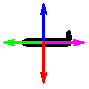
\includegraphics[width=0.3\linewidth]{figures/free-body-1.pdf} \hfill
%	\captionof{subfigure}{Angles evolution over time}
	\label{fig:free-body-1}
		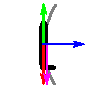
\includegraphics[width=0.3\linewidth]{figures/free-body-2.pdf}\hfill
%	\captionof{subfigure}{Angles evolution over time}
	\label{fig:free-body-2}
		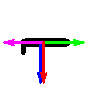
\includegraphics[width=0.3\linewidth]{figures/free-body-3.pdf}
%	\captionof{subfigure}{Angles evolution over time}
	\label{fig:free-body-3}
	\vspace{0.5cm}
%\end{minipage}

Note that at all times the lift behaves as the centripetal force, thus indicating that both the velocity and radius limitations to perform the Immelmann turn are inherent to the wing design and its maximum and minimum lift generation.\\
AS the motion will be circular, the normal and tangential accelerations will follow:
\begin{align*}
	a_n=&\frac{V^2}{R}=V\dot{\gamma}=\dot{\gamma}^2R&a_t=V^2R
\end{align*}
As a result, the radius can be writen as a function of the angle of attack. By operating with the third equation of system number \ref{eq:semicircle}, which is in wind system of reference, very convenient as is also polar system:
\begin{align*}
	L=&m\left(\frac{V^2}{R}+g\cos(\gamma)\right)\\
	\frac{1}{2}\rho S V^2 C_L(\alpha)=&m\left(\frac{V^2}{R}+g\cos(\gamma)\right)\\
	R=&\frac{2mV^2}{2W\cos(\gamma)+\rho S V^2 C_L(\alpha)}
\end{align*}
As the plane must describe a semicircle, the radius must be constant.

Plot x, z with time y despues en plano (ver trayectoria).
We can consider the maneuver coordinates:
\begin{align*}
	\dot{x}_e=&V\cos\gamma&&&	x_e=&Vt\cos\gamma \\
	\dot{y}_e=&0& \rightarrow&&	y_e=&0\\
	\dot{x}_e=&-V\sin\gamma&&&z_e=&-Vt\sin\gamma
\end{align*}

If we take both V (controlled by the gas control lever) and $\gamma$ 
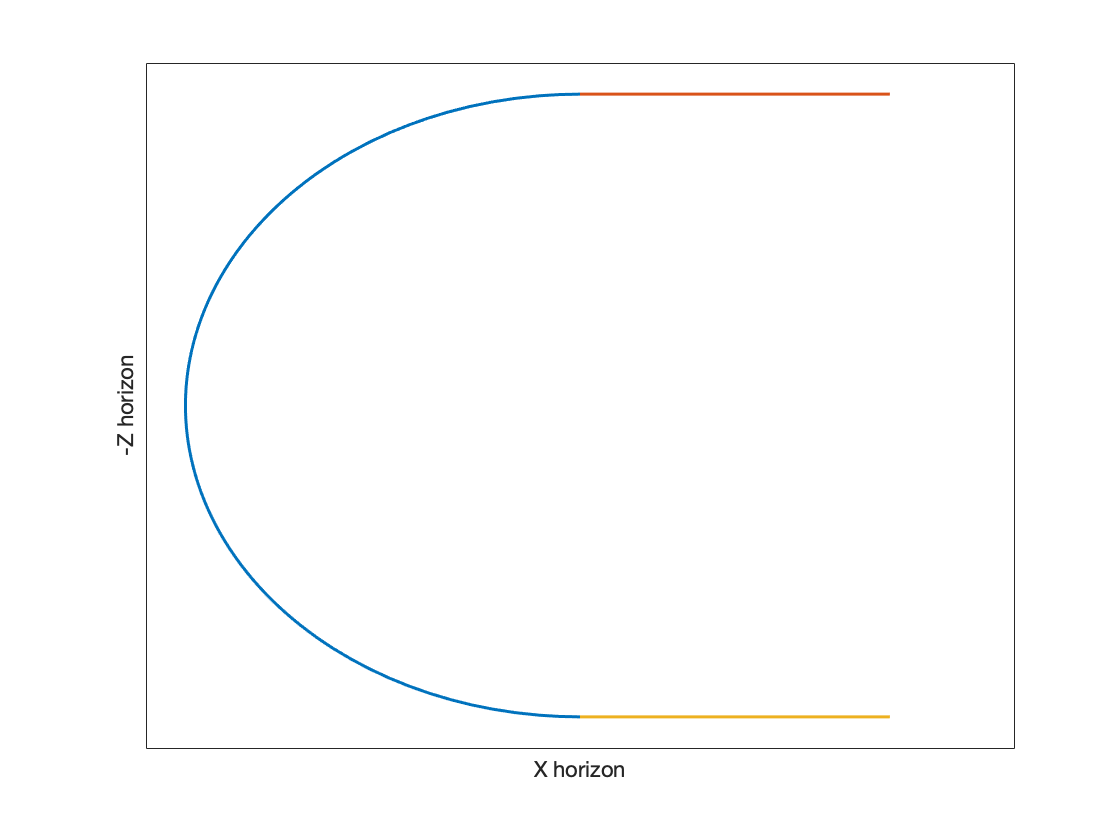
\includegraphics[width=\linewidth]{../matlab/trajectory.png}